\documentclass[11 pt]{article}

\usepackage{natbib}
\usepackage[nottoc]{tocbibind}

\usepackage[utf8]{inputenc}
\usepackage[T1]{fontenc}
\usepackage[french]{babel}

\usepackage{amsmath}
\usepackage{empheq}
\usepackage{tikz}
\usepackage{tikz-qtree}
\usepackage{listings}
\usepackage{graphicx}
\usepackage{algorithm2e}
\usepackage[left=2.5cm,right=2.5cm,top=1.5cm,bottom=1.5cm]{geometry}
\usepackage[toc,page]{appendix}
\usepackage{hyperref}
\hypersetup{
  colorlinks,
  citecolor=black,
  filecolor=black,
  linkcolor=blue,
  urlcolor=blue
}
\usepackage{appendix}
\usepackage{enumitem}           % modified itemize
\usepackage{float}
\usepackage{xcolor}
\usepackage{listings}
\lstdefinelanguage{json}{
    basicstyle=\small\ttfamily,
    numbers=left,
    numberstyle=\scriptsize,
    stepnumber=1,
    numbersep=8pt,
    showstringspaces=false,
    breaklines=true,
    frame=lines,
    backgroundcolor=\color{background},
    literate=
     *{0}{{{\color{numb}0}}}{1}
      {1}{{{\color{numb}1}}}{1}
      {2}{{{\color{numb}2}}}{1}
      {3}{{{\color{numb}3}}}{1}
      {4}{{{\color{numb}4}}}{1}
      {5}{{{\color{numb}5}}}{1}
      {6}{{{\color{numb}6}}}{1}
      {7}{{{\color{numb}7}}}{1}
      {8}{{{\color{numb}8}}}{1}
      {9}{{{\color{numb}9}}}{1}
      {:}{{{\color{punct}{:}}}}{1}
      {,}{{{\color{punct}{,}}}}{1}
      {\{}{{{\color{delim}{\{}}}}{1}
      {\}}{{{\color{delim}{\}}}}}{1}
      {[}{{{\color{delim}{[}}}}{1}
      {]}{{{\color{delim}{]}}}}{1},
}
\colorlet{punct}{red!60!black}
\definecolor{background}{HTML}{FFFFFF}
\definecolor{delim}{RGB}{20,105,176}
\colorlet{numb}{magenta!60!black}

\title{Projet Transboost}
\author{Luc Blassel, Romain Gautron}
\date{13 Mars 2018}
\linespread{1.2}
\begin{document}
\maketitle

\tableofcontents
\newpage

\section{Contexte}
\paragraph{}L’apprentissage supervisé  classique nécessite un grand nombre de données étiquetées, et dans certains cas une période de temps très importante pour pouvoir établir des modèles fiables. Ceci n’est pas toujours possible dans le monde réel, parfois il n’est simplement pas possible de collecter assez de données pour entraîner nos modèles ou alors le temps nécessaire pour l'entraînement du modèle est beaucoup trop long pour que ce soit utilisable en pratique avec des ressources conventionnelles. L’apprentissage par transfert peut nous aider à résoudre ce type de problèmes.

\paragraph{}L’apprentissage par transfert nous permet de transférer des connaissances apprises depuis domaine source avec idéalement une grande quantité de données étiquetées de bonne qualité, vers un domaine cible. Cette approche permet de réutiliser des portions d’un modèle préalablement entrainé dans notre nouveau modèle. L'avantage est double : économie en temps de calcul et utilisation d'une quantité limitée de données en réinvestissant de l'information provenant d'une autre tâche. Cette méthode est considérée comme le prochain moteur de succès de l’apprentissage automatique après l’apprentissage supervisé.

\paragraph{}La méthode TransBoost \cite{transboost}, introduite par Antoine Cornuéjols et ses collègues propose une implémentation de l’apprentissage par transfert différente de l'usage. Quand l’approche “classique” de l’apprentissage par transfert adapte l'hypothèse développée sur le domaine source au domaine cible, TransBoost en prend le contre-pied. En effet dans cette dernière on apprend l'hypothèse sur le domaine source et on projette ensuite les points du domaine cible sur le domaine source pour utiliser directement l'hypothèse source sur les points projetés.

\paragraph{}Ainsi, on n'apprend pas de nouvelles frontière entre les points, on injecte plutôt les points des bons côtés des frontières source. La projection des points du domaine cible sur le domaine source se fait dans le cadre d'un algorithme de boosting, qui grâce à plusieurs projecteurs faibles, permet d’obtenir un projecteur fort. Ce dernier permet alors d’utiliser l'hypothèse source pour classifier les points du domaine cible. La différence d'approche entre apprentissage par transfert "usuel" et Transboost est illustrée sur le schéma ~\ref{figDiff}.


\paragraph{}L'approche Transboost a d’abord été testée sur la classification des séries temporelles incomplètes et à été un franc succès en ayant de bien meilleures performances que d’autres approches du même problème. Cependant, la classification d’images étant le mètre étalon en ce moment, le but de ce projet est d’adapter la méthode TransBoost à la classification d’images en utilisant des réseaux de convolution profonds (deep CNN). Ce travail ne présente que la classification binaire d'images.

\begin{figure}[H]
  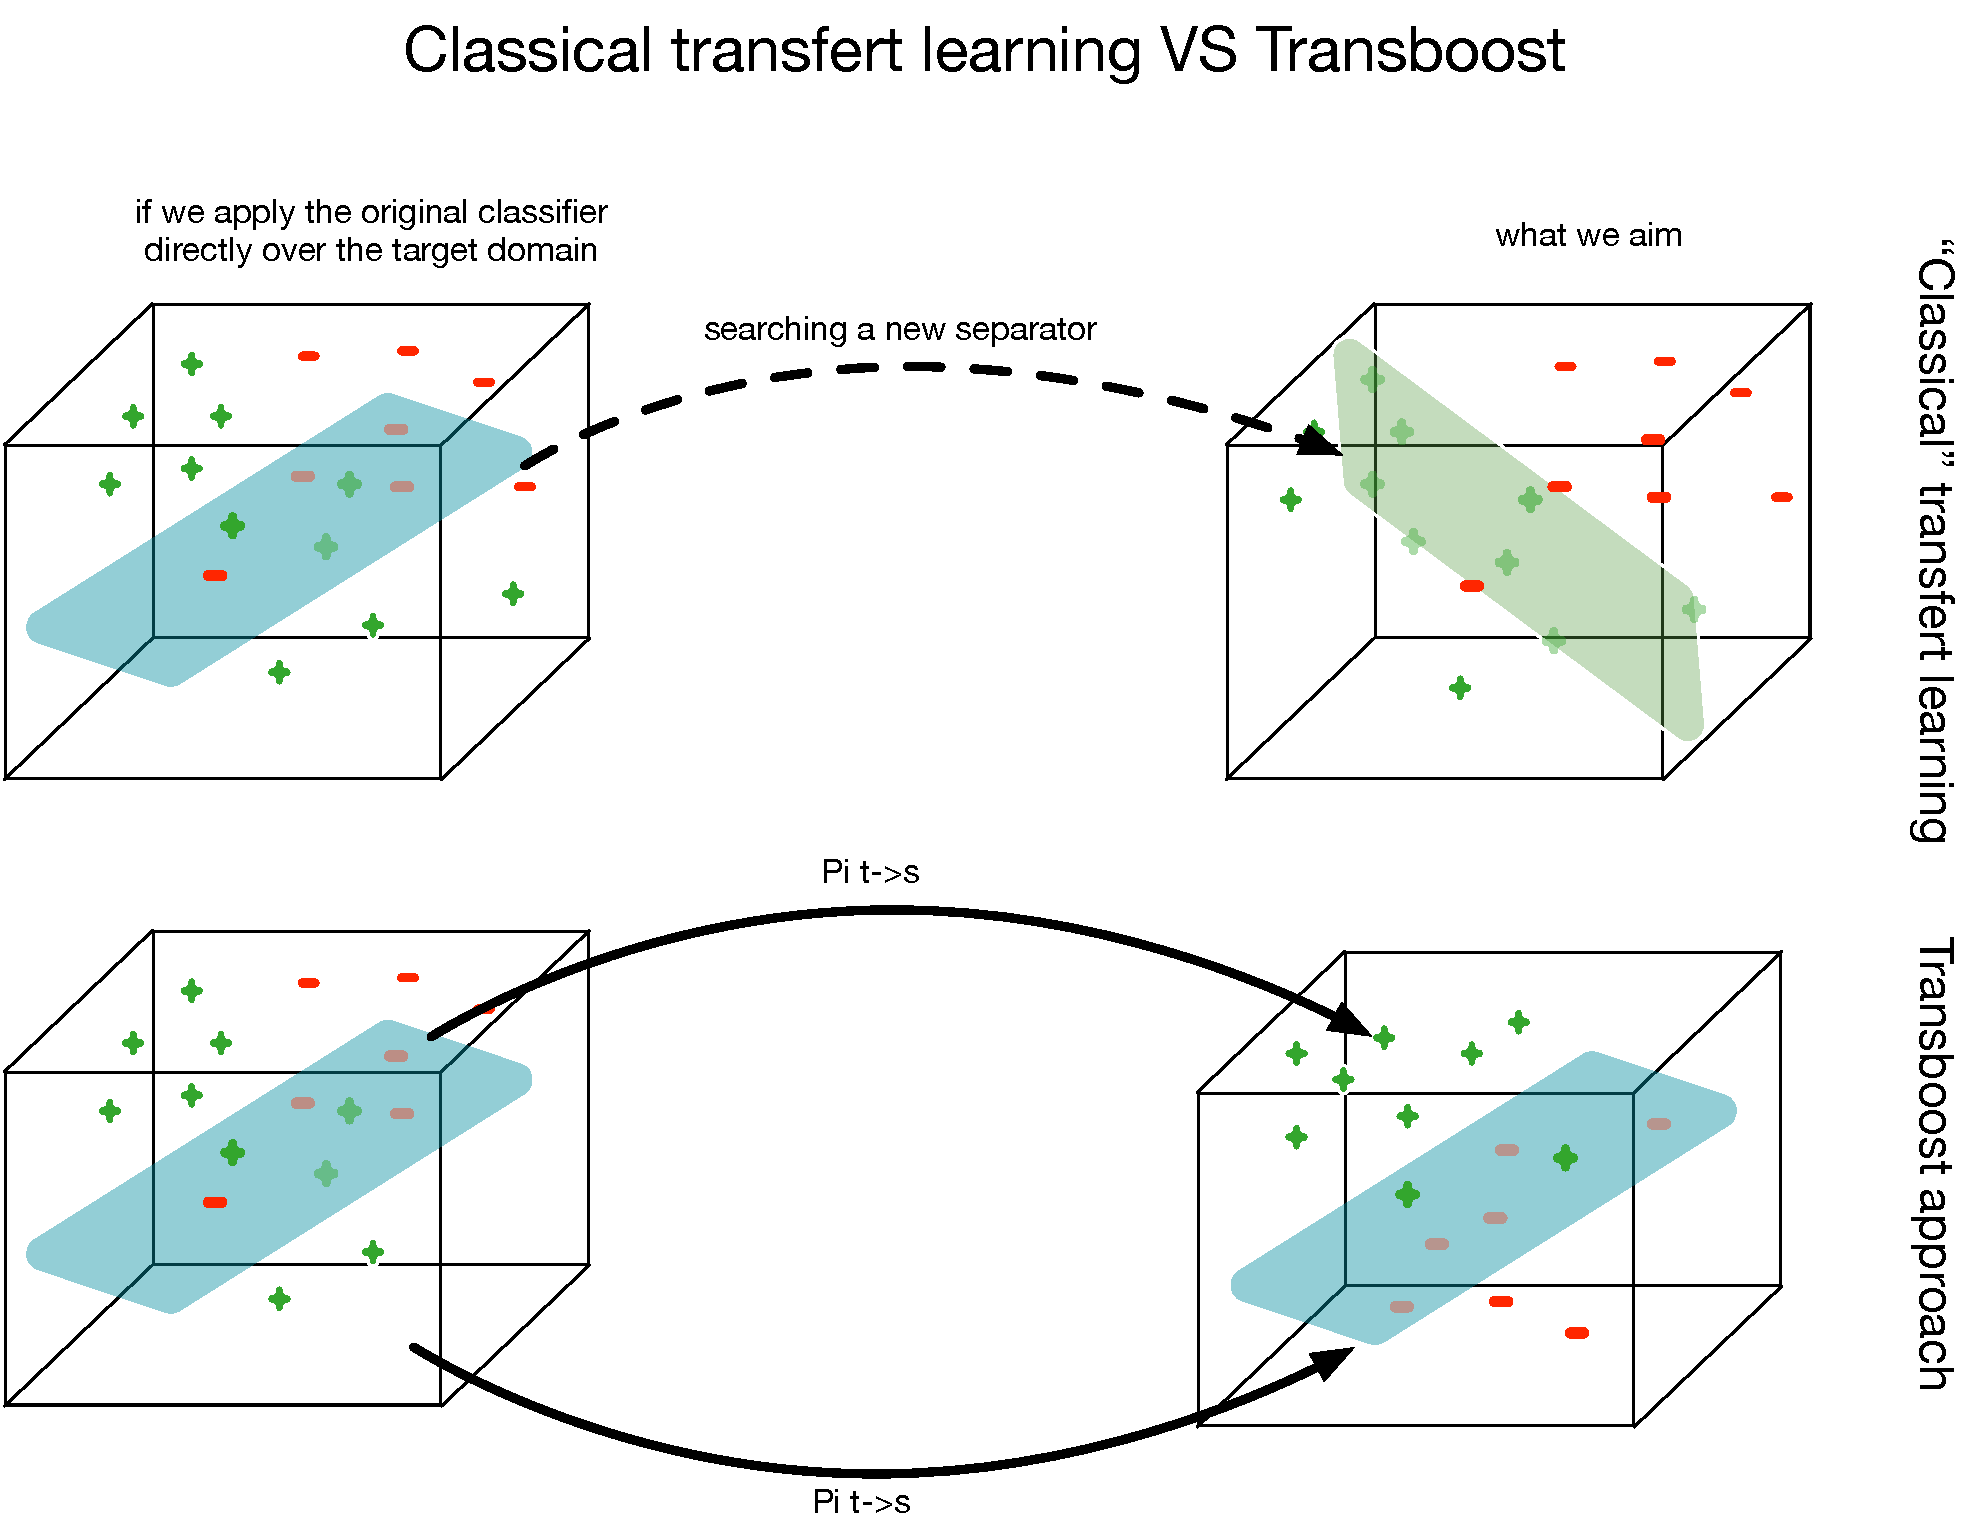
\includegraphics[width=\textwidth]{fig2.pdf}
  \caption{Différences entre l'approche classique et l'approche TransBoost}
  \label{figDiff}
\end{figure}

\section{Transboost pour la classification d'images : principe}

\paragraph{}L’application de la méthode TransBoost à la classification d’images oblige à se poser plusieurs questions. D’une part la très grande dimensionnalité des images force a utiliser des méthodes très lourdes telles que les réseaux de convolution profonds, c'est donc un défi en terme de puissance de calcul. D’autre part comment réaliser la projection des points du domaine cible dans le cas d'images ?

\paragraph{} Le choix a été fait de modifier les premières couches du réseau "source" pour classifier les images du domaine cible. Ainsi, les premières couches du réseau existant se chargeront de trouver les bons descripteurs de faible niveau pour que la nouvelle tâche puisse être réalisée. Cependant il faudra trouver les meilleurs hyper-paramètres de ces projecteurs (voir infra).

\paragraph{} On aurait pu également construire une réseau externe qui se charge d'être le projecteur des images et qui arrive en entrée du réseau "source". Celui-ci aurait eu en entrée des images et en sortie également des images (visualisation intéressante). A noter que cette option aurait été plus lourde en calculs (backpropagation supplémentaire) et ne sera pas explorée ici.

\pagebreak

\begin{samepage}
La construction d'un projecteur s'effectue comme suit : \medskip
  \begin{itemize}
    \item On obtient un réseau convolutionnel très performant sur une classification binaire source et aussi bon que le hasard pour une classification binaire cible. Les modèles pré-entraînés disponibles ont souvent un grand nombre de classes de sortie. Il est nécessaire de changer la couche de sortie du réseau et de l’entraîner pour l’ajuster à notre domaine source binaire.
    \nopagebreak
    \item On gèle la partie supérieur dudit réseau en laissant les premières couches entraînables.
    \nopagebreak
    \item On ré-entraîne ledit modèle partiellement gelé pour obtenir un projecteur en visant une valeur de métrique seuil pour arrêt. Nous choisissons la précision comme métrique, celle-ci étant parlante et pertinente dans le cas de datasets équilibrés en classes.
  \end{itemize}
\end{samepage}

On construit itérativement un ensemble de projecteurs faibles spécialisés sur les erreurs des précédents selon l'algorithme Adaboost \cite{boosting}. Notre hypothèse finale sur le domaine cible sera une combinaison linéaire de ces projecteurs faibles.

\section{Application}

Dans toute cette section, la figure~\ref{figRes} illustrera les propos.

\begin{figure}[H]
  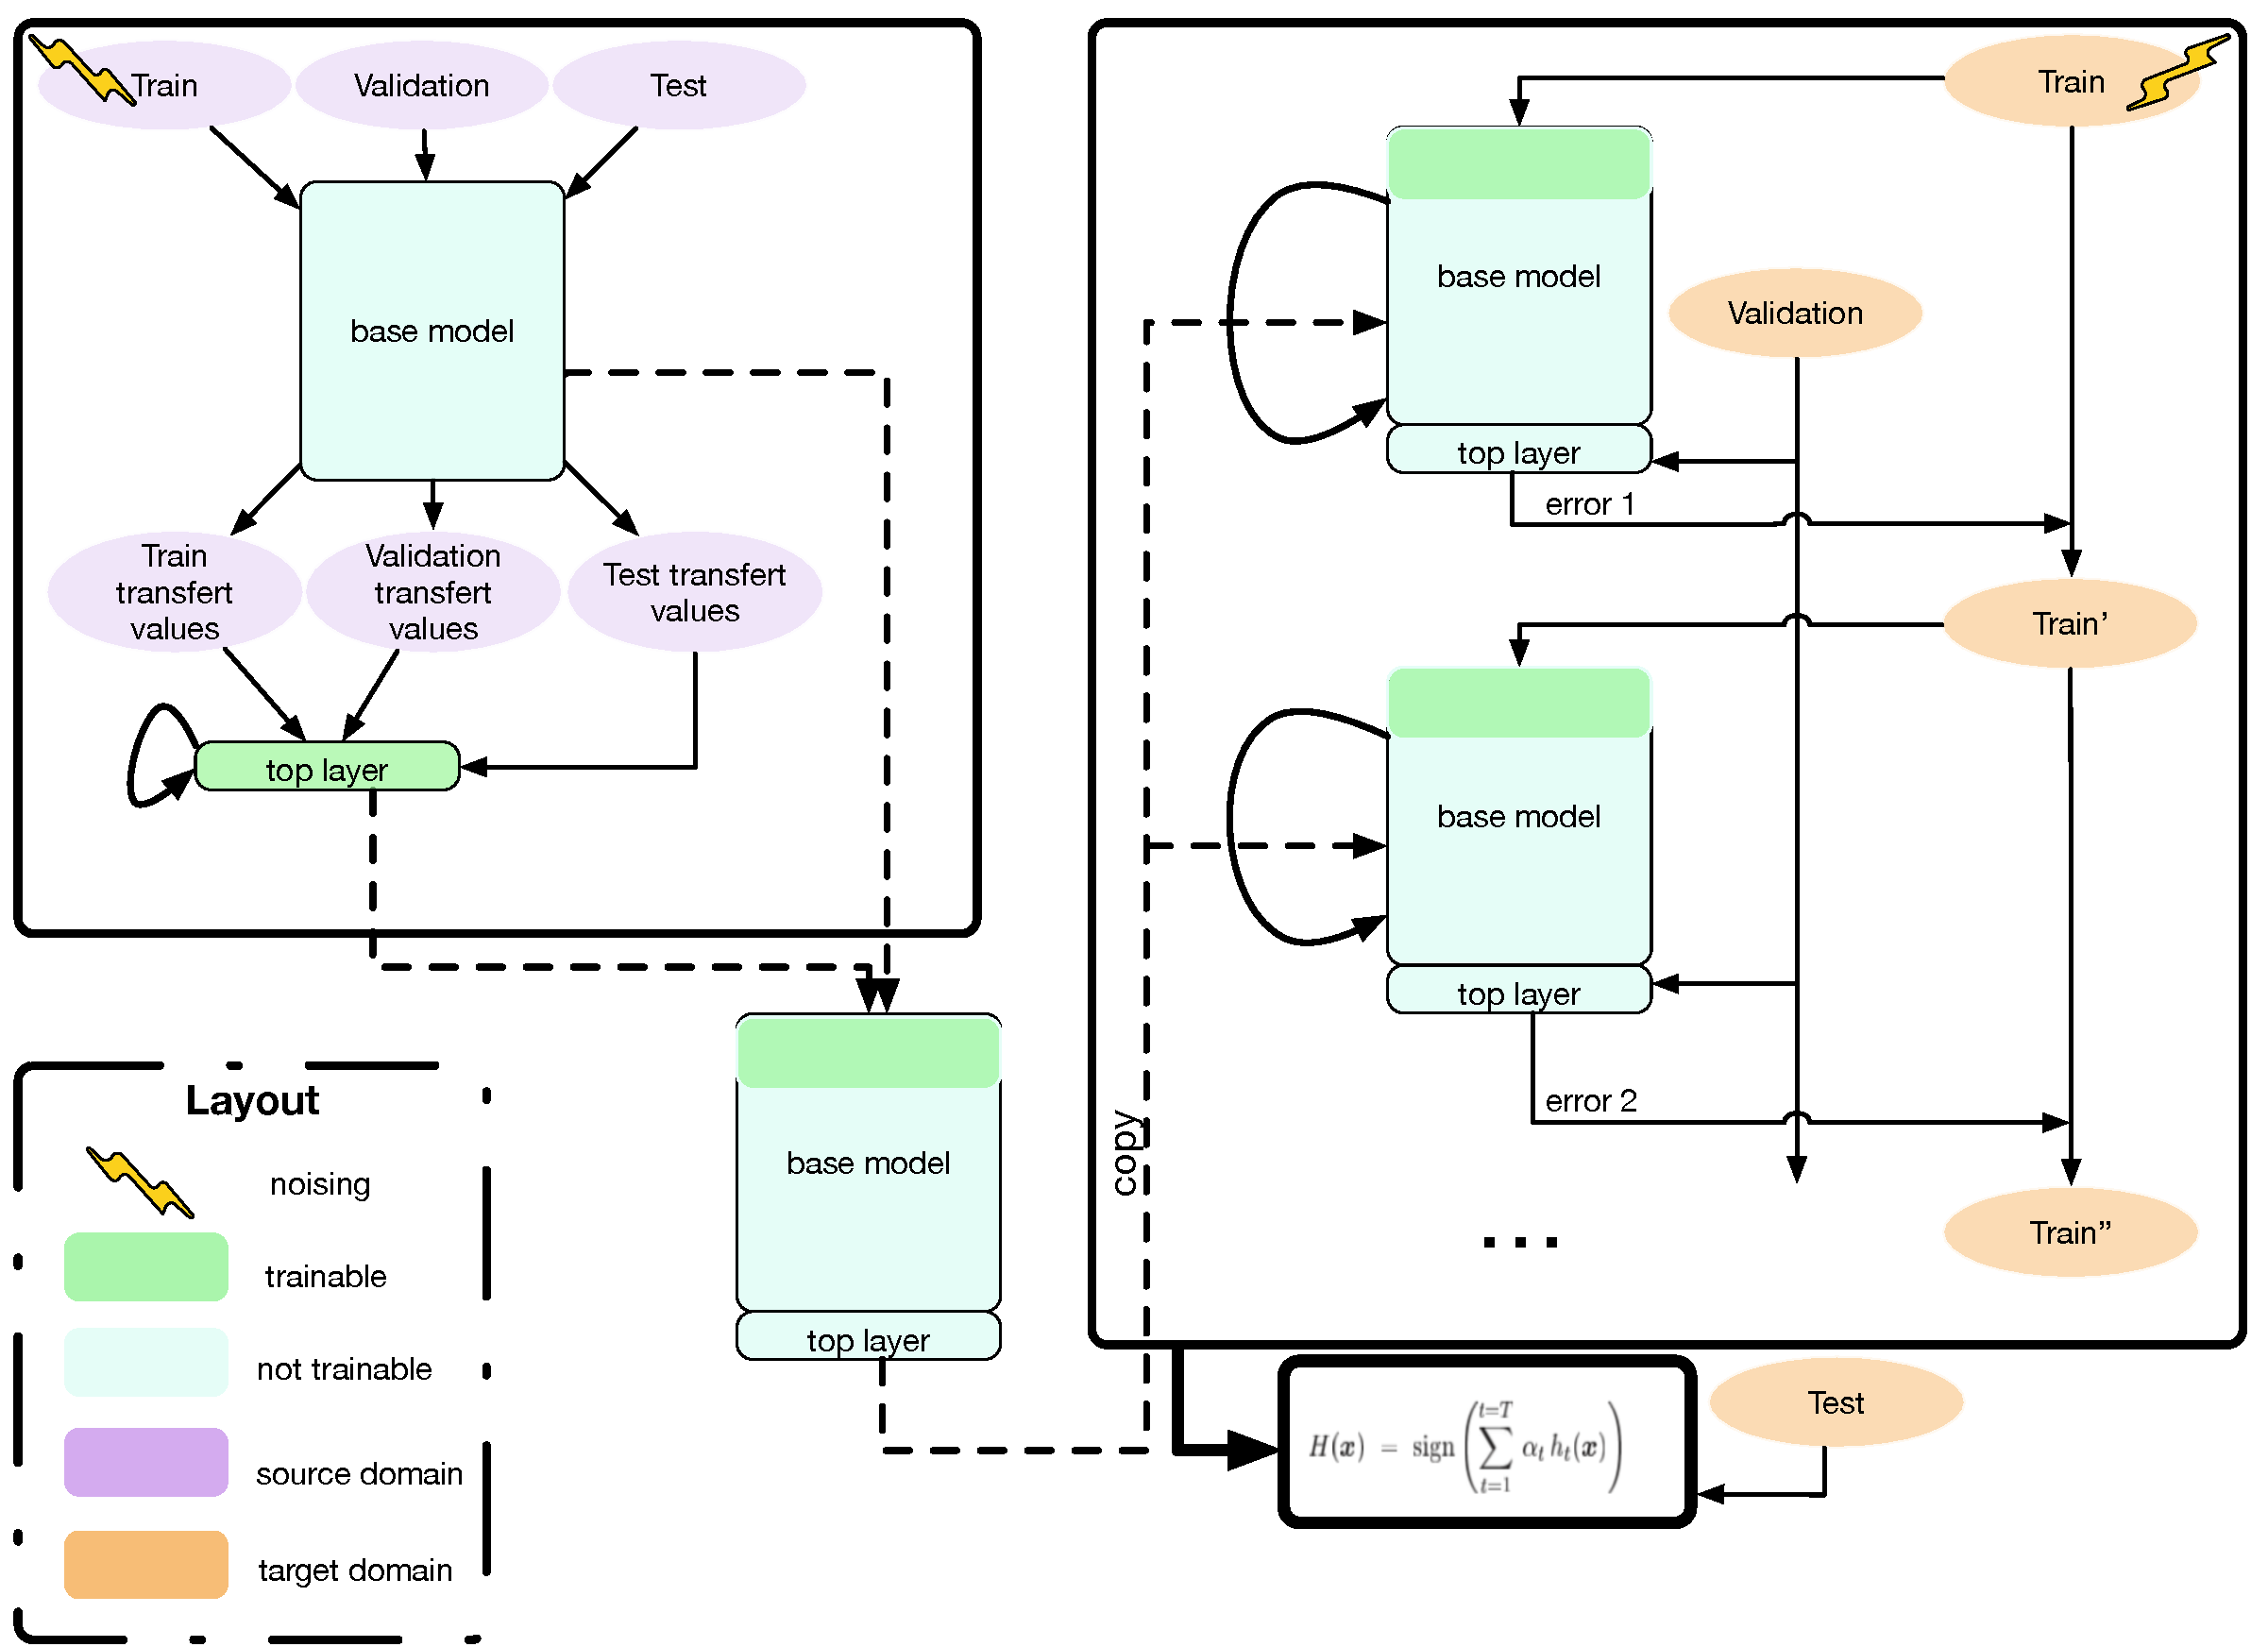
\includegraphics[width=\textwidth]{fig1.pdf}
  \caption{Déroulement de la méthode TransBoost dans le cadre de ce projet}
  \label{figRes}
\end{figure}

\subsection{Présentation des données}
\paragraph{}Nous avons choisis le jeu de données CIFAR-10 composé d’images RGB 32x32. Celui-ci est composé de 60000 images se ventilant en 10 classes (avion,automobile,oiseau,chat,cerf,chien,grenouille,cheval,bateau,camion). Les motivations pour ce choix sont :\\ \medskip
\begin{itemize}
  \item qu’il s’agit d’un jeu de données de référence usuel dans le milieu
  \item que la faible de taille des images limite le volume des données à manipuler
  \item le faible nombre de classes permet néanmoins de constituer des couples plus ou moins ardus (avion/chat vs chien/chat)
\end{itemize}

\paragraph{}Les données sont déjà reparties en 3 ensembles : entraînement, validation et test. Pour pallier au faible nombre des données dans la base d’entraînement on introduira du bruit dans celles-ci pour éviter tout sur-apprentissage. Ce bruit consiste en des rotations, zooms, déformations aléatoires. Attention, aucun bruitage n’est appliqué aux ensemble de validation et de test. En effet, on veut ceux-ci les plus représentatifs possible des images “réelles” pour éprouver le modèle.

\paragraph{}Pour constituer les ensembles source et cible, il s’agit dans les faits de simple paramètres d’entrées qui permettent de changer les classes de manière aisée (exemple : classes\_source = ['dog','truck'], classes\_target = ['deer','horse']). A noter que le bruitage des sets d’entraînement est appliqué pour les deux domaines.


\subsection{Construction d'un classificateur binaire fort sur le domaine source}
\paragraph{}Afin de pouvoir mettre en application l’idée du TransBoost, nous devons tout d’abord obtenir un classificateur binaire fort sur une tâche et aussi bon que le hasard sur une seconde. Pour cela, nous devons d’abord choisir quel sera notre modèle de base. On entend par modèle de base un réseau profond déjà entraîné et sans les dernières couches (couches connectées et softmax). \texttt{Keras} offre de nombreuses possibilités de modèles (voir \href{https://keras.io/applications/}{ce lien}). Le choix s’est porté sur le modèle Xception, d’une part pour la qualité des valeurs de transferts qu’il produit et d’autre part pour le temps qu’il faut pour générer ces valeurs de transfert. On appelle valeurs de transfert les valeurs des fonctions d’activation de la dernière couche du modèle de base pour un ensemble d’images.

\paragraph{}Par soucis de parcimonie en temps de calcul, on fait passer l’ensemble des sets d’images dans le modèle de base une seule fois. On génère ainsi les valeurs de transfert qui serviront à l’entraînement de la dernière couche. \\
L’architecture de la dernière couche (plus exactement du dernier bloc) est :\\ \medskip
\begin{samepage}
  \begin{itemize}
    \item une couche entièrement connectée de taille 1024, activation “relu”
    \nopagebreak
    \item un dropout à 50 \%
    \nopagebreak
    \item une couche entièrement connectée de taille 512, activation “relu”
    \nopagebreak
    \item un dropout à 50 \%
    \nopagebreak
    \item un couche de taille 1, activation “sigmoïd”
  \end{itemize}
\end{samepage}

\medskip

\paragraph{}Le choix de cette architecture s’est fait de manière empirique.\\

Comme pour le bruitage des images, le dropout est ici pour prévenir le sur-apprentissage compte tenu du faible nombre d’images présentées.
Une fois la dernière couche entraînée et répondant aux caractéristiques désirées, on assemble le modèle de base et ladite dernière couche en un modèle complet.


\subsection{Mise en pratique du TransBoost}
\paragraph{}Une fois que nous avons constitué notre classificateur fort, il faut voir la suite comme l’application classique d’Adaboost. La seule nuance est que, au lieu de repartir d’un classificateur “from scratch” on va cette fois partir d’un classificateur partiellement entraîné pour constituer notre projecteur faible.

\paragraph{}On cherche, non pas comme dans l'apprentissage par transfert classique avec les CNN à réapprendre une nouvelle séparatrice linéaire en entraînant la dernière couche pour une nouvelle tâche. On cherche à faire rentrer pour la nouvelle tâche les points des bons cotés de la séparatrice pour la tâche précédente en cherchant des descripteurs de faibles niveau correspondants (i.e. en ré-entraînant les premiers blocs du réseaux de neurones profond) pour que cela soit réalisé.

\paragraph{}Pour ce faire,  on prend le modèle que nous avions à l’étape précédente, on dégèle les premières couches du modèle de base et on gèle tout le reste. A ce stade deux approches sont possibles : soit réinitialiser les poids des couches dégelées soit conserver les poids. Il se peut qu’en réinitialisant le poids de ces couches avec des descripteurs de faible niveau ne permette pas à l’algorithme de converger sur si peu de données. La réponse viendra des expérimentations. Dans les deux cas, le modèle résultant de l’étape citée servira de classificateur à entraîner lors des étapes de boosting.\\

Trois paramètres importants sont à chercher selon un compromis performances/coût calculatoire :\\ \medskip
\begin{itemize}
  \item la force des classificateurs (seuil de précision) à chaque étape de boosting
  \item le nombre de blocs convolutifs à entraîner
  \item le nombre de projecteurs faibles entraînés
\end{itemize}

\paragraph{}La suite est celle de l’algorithme Adaboost (voir ~\ref{ada}). A noter que l’erreur totale du modèle est mesurée sur le set de validation. Par contre le modèle est bien entraîné sur le set d’entraînement pondéré, et la pondération des points basée sur les prédictions faites sur ce même set d’entraînement.\\

A chaque étape, l’entraînement d’un projecteur s’arrête lorsqu’un seuil de précision est atteint (avec une limite d’un grand nombre d’epochs).

\pagebreak

\begin{algorithm}[H]
  \SetAlCapSkip{10ex}
  \SetKwInOut{Input}{input}\SetKwInOut{Output}{output}
  \SetKw{Init}{Initialisation:}
  \Input{$\mathcal{X_S}\rightarrow\mathcal{Y_S}$ :  l’hypothèse source\\
          $\mathcal{S_T = \{(X_\mathrm{i}^T,Y_\mathrm{i}^T)\}}_{1\leq i\leq m}$ : l'ensemble d’entraînement cible}
  \Init{} de la distribution sur le jeu d’entraînement:$D_1(i)=1/m\ for\ i=1,\cdots,m$\;
  \For{$n=1,\cdots,N$}{
    Trouver une projection $\pi_i:\mathcal{X_T\rightarrow X_S}$ tq. $h_S(\pi_i(.))$ soit meilleure que le hasard sur $D_n(\mathcal{S_T})$\;
    Soit $\epsilon_n$ le taux d'erreur de $h_S(\pi_i(.))$ sur $D_n(\mathcal{S_T})$: $\epsilon_n = P_{i~D_n}[h_S(\pi_n(x_i))\neq y_i]$(avec $\epsilon_n<0.5$)\;{}
    Calculer $\alpha_i=\frac{1}{2}log_2(\frac{1-\epsilon_i}{\epsilon_i})$\;
    Mettre a jour: \For{$i=1,\cdots,m$}{
        \begin{equation*}
          \begin{split}
            D_{n+1}(i) & = \frac{D_n(i)}{Z_n}\times\begin{cases}
              e^{-\alpha_n}\ si\ h_{\mathcal{S}}(\pi_n(x_i^{\mathcal{T}}))=y_i^{\mathcal{T}} \\
              e^{\alpha_n}\ si\ h_{\mathcal{S}}(\pi_n(x_i^{\mathcal{T}}))\neq y_i^{\mathcal{T}}
            \end{cases}\\
            & = \frac{D_n(i)exp(-\alpha_n y_i^{(\mathcal{T})}h_{\mathcal{S}}(\pi_n(x^{(\mathcal{T})})))}{Z_n}
          \end{split}
        \end{equation*}
        Ou $Z_n$ est un facteur de normalisation tq. $D_{n+1}$ soit une distribution de $\mathcal{S_T}$\;
    }
  }
  \Output{L'hypothese finale $H_{\mathcal{T}}:\mathcal{X_T \rightarrow Y_T}$:\\
            $ H_{\mathcal{T}}(x_{\mathcal{T}})=signe\{\sum\limits_{n=1}^N \alpha_n h_{\mathcal{S}}(\pi_n(x^{\mathcal{T}}))\}$}

  \caption{Algorithme Transboost}
  \label{ada}
\end{algorithm}

\subsection{Difficultés rencontrées}
\paragraph{}Nous avons pris la décision initiale de travailler dans un environnement purement \texttt{Tensor Flow}, puisque le modèle que nous avions choisi était disponible dans cette librairie. Cependant dès qu’il a été temps de modifier la structure du modèle (pour avoir une couche de sortie binaire par exemple) ou qu’il a fallu geler l'entraînement de certaines couches l’utilisation de \texttt{Tensor Flow} est devenue très compliquée. En effet l’objet du modèle était introuvable et il fallait modifier un graphe ce qui nous a posé beaucoup de problèmes. C’est pour cela que nous avons décidé d’utiliser la librairie \texttt{Keras} qui fonctionne comme surcouche de \texttt{Tensor Flow} ce qui nous a permis d’utiliser les modèles disponible dans \texttt{Tensor Flow} mais en ayant des outils et une syntaxe plus claire et plus simple d’utilisation, permettant des temps de développement beaucoup plus courts.

\paragraph{}Nous avons aussi rencontré beaucoup de problèmes de ressources machine, puisque les machines physiques et virtuelles auxquelles nous avions accès présentaient des performances limitées. Ceci a engendré des temps d'exécution se comptant en dizaine d’heures et même en jours dans certains cas et aboutissant souvent a des erreurs de mémoire. Il est donc nécessaire d’avoir accès à une machine performante qui nous permettra débugger le programme et le perfectionner sans attendre des périodes très longues.

\paragraph{}Au fur et a mesure de l'avancement du projet et avec la mise en disponibilité d'une machine plus puissante nous avons rencontré d'autres problèmes, en effet avec la modification constante du réseau, réinitialisation des poids et sauvegarde nous avons décidé d'enregistrer les objets modèles dans une liste a chaque fin d’itération de boosting et de supprimer l'objet modèle actif avec la fonction \texttt{del} de Python. Cependant cette fonction ne garantit pas la suppression immédiate de l'objet \`a cause du système de gestion de mémoire vive de Python et même en forçant l’exécution du "garbage collector" du langage C (qui est utilise pour gérer la mémoire en Python) nous observions des comportements étranges avec des modèles qui n’étaient pas entièrement supprim\'es et donc des poids qui ne changeaient pas entre chaque étape du boosting.

\paragraph{}Nous avons au final décide d'enregistrer les modèles a chaque étape sur le disque dur de la machine avec des fonctions de \texttt{Keras} qui permettent d'une part de sauvegarder l'architecture du modèle dans un fichier \emph{.json} et les poids dans un autre. Etant donné que l'architecture du réseau ne change pas il est possible de ne l'enregistrer qu'une seule fois après l’entraînement du modèle sur l'espace source. Cette architecture indique également quelles couches sont entraînable lors de la phase de boosting, et par la suite a chaque fois que l'on souhaite enregistrer le modèle on peut se contenter d'enregistrer uniquement les poids. 

\paragraph{}Une fois que le modèle est sauv\'e sur le disque dur on peut appeler une fonction de \texttt{Tensor Flow} qui permet d'effacer tous les objets de la session \texttt{Tensor Flow} et ainsi s'assurer que plus aucun objet modèle précédemment entraîne ne persiste et ne perturbe l’entraînement de nouveaux modèles. Pour pouvoir entraîner un nouveau modèle il suffit, a chaque début d’itération de boosting de créé un réseau a partir de l'architecture sauvée sur disque et d'y charger les poids du modèle de base.

\paragraph{} Une fois que tous les projecteurs ont été entraînés on peut effectuer les prédictions en chargeant séquentiellement chaque modèle (en chargeant l'architecture et les poids) et d'enregistrer ses prédictions avant de supprimer le modèle et de charger le suivant. A la fin la liste de prédiction est pondérée avec les $\alpha$ calcul\'es lors du boosting et on obtient la prédiction finale issue du boosting

\paragraph{} \emph{A priori} cette méthode de tout enregistrer sur le disque avant de tout supprimer et tout recharger peut paraître lourde et pas forcement nécessaire, cependant ces étapes supplémentaires et le temps d’accès beaucoup plus long du disque dur par rapport a la mémoire vive sont de petits prix a payer par rapport a la garantie que l'on entraîne bien ce que l'on veut entraîner et qu'il ne peut pas y avoir de "contamination" entre les étapes du boosting. 

\section{Comparaisons critiques portant sur la méthode transboost}
\subsection{Projecteurs faibles vs. projecteurs forts}
\paragraph{}On veut comparer l’approche TransBoost avec faisant varier la force des projecteurs aux extrêmes. Si l’on obtient des performance supérieures avec un seul projecteur fort (i.e. les premiers groupes de couches convolutives entraînées aux maximum) alors on ne peut pas montrer un intérêt de travailler avec une multitudes de projecteurs faibles en boosting dans ce cadre précis.

\subsection{Projecteurs vs. nouveaux classificateurs}
\paragraph{}Comme on le voit, la méthode du TransBoost appliquée avec le modèle complet (base et dernier bloc) est très gourmande en temps et en espace. En effet, après avoir entraîné un grand nombre de classificateurs il faut également stocker tous ceux-ci à fin de pouvoir réaliser les classification de nouveau points selon l’hypothèse finale. En fait, on peut être plus économe en espace. En effet, il suffit de la connaissance pour reconstruire tous les modèles issus du boosting :\\ \medskip
\begin{itemize}
  \item du modèle complet non modifié
  \item uniquement pour chaque étape de boosting du poids des couches modifiées
\end{itemize}
\paragraph{}On souhaite mettre en compétitions deux approches : le TransBoost et une méthode de boosting classique.

\paragraph{}On peut atteindre un seuil de précision relativement bas à chaque étape ( de l’ordre de 0.7) simplement à l’aide d’un petit réseau convolutif initialisé (quelques blocs). Bien qu’avec l’économie en espace citée précédemment il n’y ait pas beaucoup de différence, l’économie en temps de calcul est bien là. En effet pour chaque prédiction à faire, le passage dans le petit CNN suffit. Tandis qu’à chaque étape avec le modèle de base augmenté du dernier bloc il faille calculer les activations dans toute la partie supérieure gelée du réseau avant de "backpropager" l’erreur.

\section{Conditions et méthodes d’expérimentation}
Toutes les expérimentations ont été faites sur une machine à 8 cœurs, 30 Go de mémoire RAM et 11 Go de GPU. Il s'agit d'un serveur Ubuntu avec Keras GPU. Nous avons utilisé le service Google Cloud. On interagit en lignes de commandes : on lance le programme dans un screen qui écrit un fichier \textit{.log}. On peut alors détacher le screen et quitter la machine virtuelle et revenir consulter le log en cours de construction quand l'on souhaite.

\paragraph{}Le programme est construit tel que suit : la configuration à faire tourner est spécifiée dans un fichier \textit{.json} à part (cf. \ref{config}). De par la nature des expérimentations qui étaient prévues, le programme permet également d'appeler une liste de configurations pour par exemple tester différents seuils de projecteurs.

\pagebreak 
\begin{lstlisting}[language=json,firstnumber=1,caption={Exemple de configuration},label={config}][H]
{
  "models_path" : "models",
  "models_weights_path" : "models_weights",
  "path_to_best_model" : "best_top_model.hdf5",
  "threshold" : 0.65,
  "proba_threshold" : 0.5,
  "transformation_ratio" : 0.05,
  "originalSize" : 32,
  "resizeFactor" : 5,
  "batch_size_source" : 10,
  "batch_size_target" : 10,
  "epochs_source" : 1000,
  "epochs_target" : 1000,
  "classes_source" : ["dog","truck"],
  "classes_target" : ["deer","horse"],
  "layerLimit" : 15,
  "times" : 1,
  "lr_source" : 0.0001,
  "lr_target" : 0.0001,
  "step" : 3,
  "recompute_transfer_values" : false,
  "train_top_model" : false,
  "reinitialize_bottom_layers" : false,
  "bigNet" : true,
  "verbose" : true
}
\end{lstlisting}

\section{Resultats}
\subsection{Construction du classificateur binaire}
\paragraph{}Dans les faits, pour la base d’apprentissage “chien/camion”, l’algorithme arrive à 98.9\% de précision sur le set de test en seulement 2 epochs. D’un autre côté ce même modèle entraîné sur le dataset précédent a un précision de 50\% en prédiction sur le dataset “deer/horse”, ce qui répond bien à ce que l’on recherchait.

\subsection{Boosting classique sur petit CNN}
\paragraph{}

\begin{figure}[H]
\begin{center}
\centerline{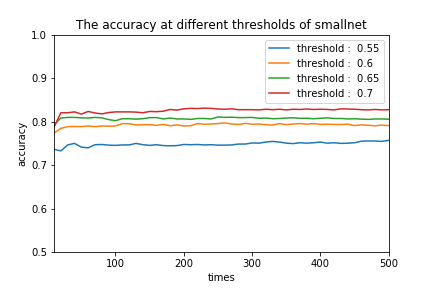
\includegraphics[width=\textwidth]{smallnet.png}}
\caption{Évolution de la précision de l'algorithme de Boosting avec des petits réseaux de convolution (sans transfert) }
\label{fig:smallNet}
\end{center}
\end{figure}

\begin{samepage}
On a construit un simple réseau de neurones de convolution  qui apprend directement la domaine cible avec l'algorithme de Boosting, sans l'apprentissage de transfert. Son architecture est:\\ \medskip \nopagebreak
  \begin{itemize}
    \item deux couches de convolution avec 32 filtres de taille 3*3 chacun, activation “relu”, max-pooling de taille 2*2
    \nopagebreak
    \item une couche de convolution avec 64 filtres de taille 3*3 chacun, activation “relu”, max-pooling de taille 2*2
    \nopagebreak 
    \item une couche flatten 
    \nopagebreak
    \item une couche entièrement connectée de taille 64, activation “relu”
    \nopagebreak
    \item un dropout à 50 \%
    \nopagebreak
    \item une couche entièrement connectée de taille 34, activation “relu”
    \nopagebreak
    \item un dropout à 50 \%
    \nopagebreak
    \item un couche de sortie avec une activation sigmoïde
  \end{itemize}
\end{samepage}
\paragraph{} On utilise ce petit réseau de convolution \`a la place des projecteurs dans l'algorithme de boosting, et on mesure la précision de classification sur le set de test \`a différentes itérations du boosting. Les résultats de cette analyse sont visibles sur la figure \ref{fig:smallNet}. Les mesures ont été effectuées pour plusieurs seuils de précision d’entraînement lors du boosting.
\paragraph{}Le set à apprendre est relativement difficile : il s'agit de "deer/horse".Ceci montre que l'algorithme de boosting a été correctement implémenté (au moins 10 points de gain de précision par rapport au seuil des projecteurs faibles). On peut voir que plus le projecteur est fort, plus la précision augmente. Au bout d'une dizaine de projecteurs on a ensuite une évolution très lente de performances.

\subsection{Méthode transboost}

Après plusieurs essais (learning rate, optimiseur, réinitialisation des couches modifiées ou non ...) l'algorithme ne converge pas ou bien pas dans un temps raisonnable. Pour que l'algorithme marche dans le boosting, celui ci doit au moins converger au seuil à la première itération assurant ainsi une performance supérieure ou égale lors du boosting. 

\bigskip

Dans les conditions présentées (30 Go de RAM, 11 Go de GPU et 8 coeurs) l'algorithme ne converge pas à un seuil de 55\% sur le set de validation au bout de 4h et ne peut dépasser 65 \% sur le set d'entraînement. Ainsi, même si l'on vise un seuil de 70\% en resubstitution pour atteindre entre 55\% et 60\% sur le set de validation, on ne pourra pas atteindre ces valeurs dans le 4h. Par conséquent on n'obtient que des projecteurs équivalents au hasard.

\bigskip
Même si l'algorithme arrivait à converger, s'il faut 4h par projecteur avec de telles ressources, on voit que cela est prohibitif. On peut expliquer cela par le fait qu'on déstabilise sur très peu de données les couches basses qui ont appris des descripteurs de faible niveau (les plus longs à apprendre). Il faut mettre ceci en regard du très peu de temps et de ressources calculatoires que nécessite le transfert learning classique avec de très bonnes performances.

\section{Expérimentations non réalisées}
Expérimentations impossibles du fait que l'algorithme ne converge pas (ou du moins en un temps raisonnable).
\subsection{Influence des domaines source et cible}
\paragraph{}Peut t-on partir d’un domaine source simple (ex : “dog/truck”) pour aller vers un domaine cible plus compliqué (ex:”deer/horse”) ? 
%====
Dans notre cas, nous souhaitons d'étudier le cas compliqué. Mais on peut aussi essayer d'autres cas. Notre objectif est vérifier la méthode de transboost, comme le domaine cible est assez compliqué, on n'a pas de preuve qu'il ne marche pas. Par contre, on pourra établir de modèle à partir d'un domaine source compliqué (ex:"deer/horse"),et l'appliquer sur le domaine cible (ex:"dog/truck")
%====
\subsection{Influence des hyper-paramètres: recherche d'un optimum précision/coût calculatoire}
\begin{itemize}
\item Influence de la force des projecteurs
\item Influence du nombre de projecteurs
\item Influence du nombre de blocs entraînés.\emph{(Dans l’idéal on veut en modifier le moins possible pour atteindre au plus vite le seuil de précision)}
\end{itemize}

\subsection{Transboost vs classical transfer learning}
\paragraph{}Pour un domaine cible difficile (deer/horse), on arrive sans fine-tuning à une précision de 92.6\% en moins de 10 epochs. Ce résultat peut être grandement amélioré à l'aide d'un "fine tuning" des derniers blocs convolutifs du modèle de base. 

\section{Conclusion}
Si l'idée du transboost semble prometteuse dans le cadre des séries temporelles, l'application à la classification d'images avec ses problématiques inhérentes (taille de données et difficulté de classification) ne semble pas probante.

\paragraph{} Comme on le présageait l'implémentation transboost nécessite de capacité de calcul très importantes. Le fait que l'algorithme ne converge pas (sauf erreur de notre part) ou bien pas dans un temps raisonnable ne justifie pas de poursuivre les expérimentations telles que nous les avons abordées. On pourrait par exemple créer un réseau à part entière qui sert de projecteur avec entrée et en sortie des images. Cependant, là encore il faudrait parcourir tout le réseau convolutionnel de base à chaque fois pour remonter l'erreur. 

\bigskip
\nocite{*}
\bibliographystyle{plain}
\bibliography{biblio.bib}

\pagebreak
\begin{appendices}
  \section{Code}
    Le code est disponible sur \href{https://gitlab.com/zlanderous/transboost}{gitlab.} avec le compte d'utlisateur suivant:
    \begin{itemize}
    	\item email: transboostproject@gmail.com
        \item password: transboostAPT2018
    \end{itemize}

  \section{Schéma du programme}
  \begin{figure}[h]
    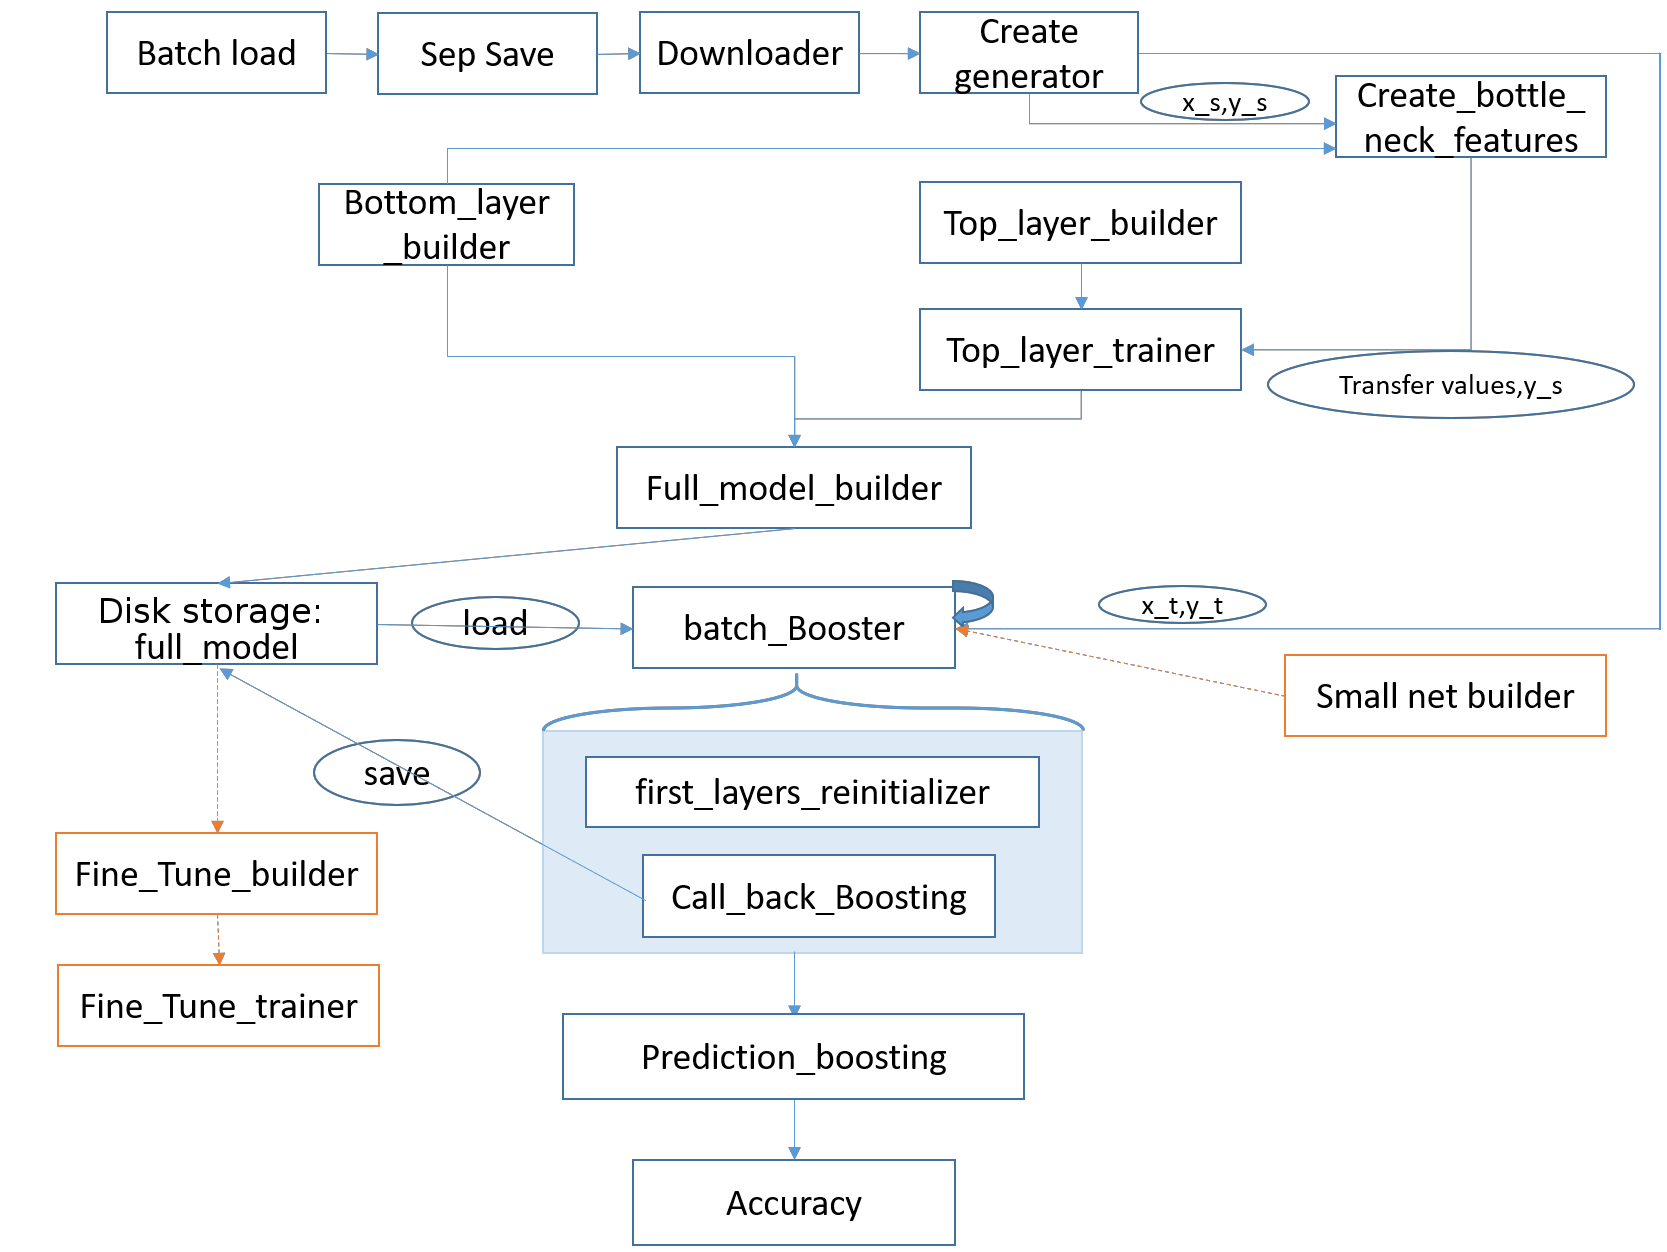
\includegraphics[width=\textwidth]{schema.png}
    \caption{schéma du programme}
    \label{figTot}
  \end{figure}
  
  \subsection*{Descriptif des fonctions}

  \begin{description}
    \item[Batch\_loader:] Prend les images d'un batch de CIFAR-10 et les enregistre dans un dictionnaire avec comme clé la classe de l'image.
    \item[Sep\_saver:] Parcourt le dictionnaire et enregistre les images de chaque classe dans un dossier correspondant.
    \item[Downloader:] Télécharge les batches de CIFAR-10 et exécute les deux fonctions précédentes pour chaque batch d’entraînement, de test et de validation.
    \item[Create\_generator:] Crée des objets de type générateur qui contiennent des batches d'images avec du bruit.
    \item[Bottom\_layer\_builder:] Charge et construit le modèle sans dernière couche (Xception dans ce cas).
    \item[Create\_bottleneck\_features:] Calcule les valeurs de transfert pour chaque image des jeux d’entraînement, de test et de validation passant par le modèle issu de la fonction précédente.
    \item[Top\_layer\_builder:] Construit la couche de sortie binaire.
    \item[Top\_layer\_trainer:] Entraîne la dernière couche avec les valeurs de transfert.
    \item[Full\_model\_builder:] Assemble le modèle sans dernière couche et la dernière couche nouvellement entraînée.
    \item[first\_layers\_reinitilizer:] Gèle les poids des $n$ dernières couches pour effectuer le boosting.
    \item[Callback\_boosting:] est appelé à chaque epoch de l’entraînement du modèle et si la précision est supérieure à un seuil $\alpha$ arrête l'entraînement et sauvegarde le modèle sur le disque dur.
    \item[batchBooster:] Applique l'algorithme adaboost au réseau. chaque modèle entraîne faisant office de projecteur faible est construit puis entraîne en appelant les deux fonctions précédentes $n$ fois.
    \item[Prediction\_boosting:] Effectue une prédiction sur la classe de l'image présentée en prenant en compte les modèles entraînés dans la fonction précédente.
    \item[Accuracy:] Évalue la précision des prédictions.
    \item[small net builder:] Construit un petit CNN avec 3 couches convolutives et 3 couches entièrement connectées avec décrochement
    \item[fine\_tune\_builder:] Construit un modèle de fine tuning. Il prend les valeurs en utilisant le modèle précédent de domaine de source.
    \item[fine\_tune\_trainer:] Entraîne le modèle de fine tuning.
  \end{description}
\end{appendices}

\end{document}

